\documentclass[10pt,letterpaper]{article}
\usepackage[top=0.85in,left=2.75in,footskip=0.75in]{geometry}

% amsmath and amssymb packages, useful for mathematical formulas and symbols
\usepackage{amsmath,amssymb}

% Use adjustwidth environment to exceed column width (see example table in text)
\usepackage{changepage}

% Use Unicode characters when possible
\usepackage[utf8x]{inputenc}

% textcomp package and marvosym package for additional characters
\usepackage{textcomp,marvosym}

% cite package, to clean up citations in the main text. Do not remove.
\usepackage{cite}

% Use nameref to cite supporting information files (see Supporting Information section for more info)
\usepackage{nameref,hyperref}

% line numbers
\usepackage[right]{lineno}

% ligatures disabled
\usepackage{microtype}
\DisableLigatures[f]{encoding = *, family = * }

% color can be used to apply background shading to table cells only
\usepackage[table]{xcolor}

% array package and thick rules for tables
\usepackage{array}

% enumerate package lets us use letters instead of numbers
\usepackage{enumerate}

% create "+" rule type for thick vertical lines
\newcolumntype{+}{!{\vrule width 2pt}}

% create \thickcline for thick horizontal lines of variable length
\newlength\savedwidth
\newcommand\thickcline[1]{%
  \noalign{\global\savedwidth\arrayrulewidth\global\arrayrulewidth 2pt}%
  \cline{#1}%
  \noalign{\vskip\arrayrulewidth}%
  \noalign{\global\arrayrulewidth\savedwidth}%
}

% \thickhline command for thick horizontal lines that span the table
\newcommand\thickhline{\noalign{\global\savedwidth\arrayrulewidth\global\arrayrulewidth 2pt}%
\hline
\noalign{\global\arrayrulewidth\savedwidth}}

\usepackage{color}

% Remove comment for double spacing
%\usepackage{setspace}
%\doublespacing

% Text layout
\raggedright
\setlength{\parindent}{0.5cm}
\textwidth 5.25in
\textheight 8.75in

% Bold the 'Figure #' in the caption and separate it from the title/caption with a period
% Captions will be left justified
\usepackage[aboveskip=1pt,labelfont=bf,labelsep=period,justification=raggedright,singlelinecheck=off]{caption}
\renewcommand{\figurename}{Fig}

% Use the PLoS provided BiBTeX style
\bibliographystyle{plos2015}

% Remove brackets from numbering in List of References
\makeatletter
\renewcommand{\@biblabel}[1]{\quad#1.}
\makeatother

% Leave date blank
\date{}

% Header and Footer with logo
\usepackage{lastpage,fancyhdr,graphicx}
\usepackage{epstopdf}
\pagestyle{myheadings}
\pagestyle{fancy}
\fancyhf{}
\setlength{\headheight}{27.023pt}
\lhead{
\includegraphics[width=2.0in]{PLOS-submission.eps}}
\rfoot{\thepage/\pageref{LastPage}}
\renewcommand{\footrule}{\hrule height 2pt \vspace{2mm}}
\fancyheadoffset[L]{2.25in}
\fancyfootoffset[L]{2.25in}
\lfoot{\sf PLOS}


%% Define per-paper macros.
\newcommand{\rulemajor}[1]{\section{#1}}
\begin{document}
\vspace*{0.2in}

\begin{flushleft}
{\Large
\textbf\newline{Ten Simple Rules for Thinking Like a Programmer}
}
\newline
\\
{Greg~Wilson}\textsuperscript{1,*}
\\
\textbf{1} RStudio, Inc. / greg.wilson@rstudio.com
\\
\bigskip
* Corresponding author.
\end{flushleft}

\section*{Abstract}

We describe ten ways experienced programmers view the world that are often
useful in other contexts.

\section*{Author Summary}

Experienced programmers often think about problems in ways inspired by their
understanding of software and software development.  Understanding how can help
people in other domains see their problems with fresh eyes.

\section*{Introduction}

Ever since \cite{Wing2006} introduced the term ``computational thinking'' in
2006, computer scientists and educators have debated what exactly it means
\cite{Denn2017}.  What isn't debated is the fact that experienced programmers
tend to think about problems in ways inspired by their experience of
programming.  This paper describes ten of those ways which may help people in
other domains see their own problems with fresh eyes.

\subsection*{Acknowledgments}

An early version of this paper was inspired by Jon Udell's essay ``Seven Ways to
Think Like the Web'' \cite{Udel2011}.

\rulemajor{Programs are data.}

The key insight that all of modern computing is built on is that programs are
just another kind of data.  Source code is text, no different from a thesis or a
poem; it can be searched with the same tools used to search other kinds of
documents, and new text (such as documentation) can be generated from old.

More importantly, once a program is loaded into memory its instructions are just
bytes, no different in principle or practice from those used to represent the
pixels in an image or the numbers in a vector field.  Those blocks of
instructions can be stored in data structures, passed to functions, or altered
on the fly, just like other data.  Almost all advanced programming techniques
depend on this fact, from function pointers in C and callbacks in JavaScript to
decorators in Python and lazy evaluation in R.

\rulemajor{Computers don't understand anything.}

Computers don't understand: they only obey instructions that make them appear
to.  If a person looks at this image, they see the word ``data'':

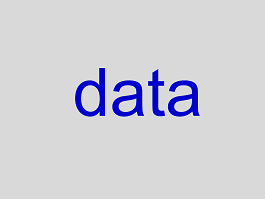
\includegraphics[width=5.0cm]{data.png}

\noindent
A machine doesn't; it doesn't even see four blobs of blue pixels on a gray
background, because it doesn't ``see'' anything.  Equally, calling a variable
``temperature'' doesn't mean the computer will store a temperature in it---it
would do exactly the same thing if the variable was called ``pressure'' or
``frankenstein'' or ``a7''.  This may seem obvious once you have written a few
programs, but thirty years after \cite{Pea1986} first called it the
``superbug'', believing that the computer will somehow understand intent remains
a common error.

\rulemajor{Programming is about creating and combining abstractions.}

Computers don't have to understand instructions in order to execute them, but we
do in order to create them (and fix them afterward).  Since our working memory
can only juggle a handful of things at once \cite{Mill1956}, we have to create
abstractions so that our representations of problems will fit into hardware
whose performance doubles over millions of years rather than every eighteen
months.

The key to making workable abstractions is to separate ``what'' from ``how'', or
in computing terms, to separate \emph{interface} and \emph{implementation}.  An
interface is what something knows how to do; its implementation is how it does
those things.  There can be dozens of different implementations of a single
interface: if we do our work well, we shouldn't have to care about the
differences between them until something goes wrong or we need to improve its
performance.

\rulemajor{Every redundancy in software is an abstraction trying to be born.}

The history of programming is in part the history of people noticing patterns
and then making it easier for programmers to use them.  Does your program
repeatedly search an array to find the largest and smallest values?  Write a
function called \texttt{bounds}.  Does it repeatedly search arbitrary data
structures to find values that meet certain criteria?  Write a generator that
returns values one by one and another function that filters those according to
some criteria.

The problem with eliminating redundancy is that it can make software denser,
which in turn makes it harder for non-specialists to understand.  Like
mathematics and modern art, it can take years of training for someone to reach
the point where they can see how beautiful something is.

The other problem with patterns is that they can lead to expert blind spot
\cite{Nath2003}.  Once experts have internalized patterns, they are often unable
to remember that they ever saw the world any other way, or to see the world
afresh through novice eyes.  As a result, they are prone to say, ``It's
obvious,'' and then follow it with incomprehensible jargon.

\rulemajor{Create models for computers and views for human beings.}

One consequence of the second and third rules is important enough to be a rule
in its own right: we should create models for computers and views for human
beings.  A \emph{model} is a precise, detailed representation of information
that is easy for a computer to operate on; a \emph{view} is a way of displaying
information that human beings can easily understand and interact with.  For
example, an HTML page is represented in memory as a data structure containing
nodes for elements like headings and paragraphs, which can in turn contain a mix
of other nodes or text:

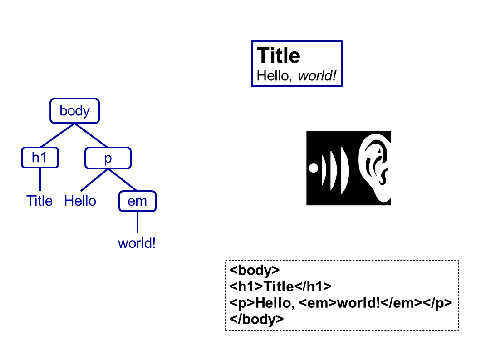
\includegraphics[width=10.0cm]{modelview.png}

\noindent
That model can be rendered in a browser, turned into speech, or displayed as
text using angle brackets.  None of these \emph{is} the model: they're all views
that make the information in the model comprehensible in different ways.

Turning a model into a view is hard, but turning a view back into a model is
harder.  For example, parsing the textual representation of HTML takes thousands
of lines of code, but doing OCR or speech recognition to translate a rendered
page or its spoken equivalent back into nodes and text can take millions.
Ironically, the same programmers who insist on this separation in software they
build for the rest of humanity have been remarkably resistant to the idea of
adopting any kind of model-view separation in programming itself.

\rulemajor{Paranoia makes us productive.}

``I want to count the cells in this photograph'' is easy to say, but what does
it actually mean?  What constitutes a cell?  When do you decide that a lumpy
blob of pixels is two cells rather than one, or three instead of two?  Every
program embodies decisions like these; the sooner these decisions are made
explicit and the earlier they're checked, the more productive we will be.  The
precise order of steps doesn't seem to matter: we can write tests, then write
software to make those tests pass, or write the program first and then test it.
What \emph{does} matter is alternating development and testing in short
interleaved bursts \cite{Fucc2017}.

Of course, we don't stop worrying once we've typed our code in.  We check that
data is formatted properly to protect ourselves against ``garbage in, garbage
out''.  We put checks in our code to make sure that parameters are sensible,
data structures consistent, files aren't empty, and so on.  This is called
\emph{defensive programming}, and one of the signs of a mature programmer is a
high density of assertions and other self-checks in her code.  It is harder to
do this in research software than in most commercial software because (almost by
definition) we don't know what the right answer \emph{is} in research software,
which makes it difficult to check that we're getting it.

\rulemajor{Things that don't change are easier to understand than things that do.}

Programmers use the words \emph{mutable} and \emph{immutable} to refer to things
that can be modified after they are created and things that cannot.  Immutable
things are easier to understand because you don't have to re-trace their history
in order to understand their state.  However, immutable data can be less
efficient than mutable data: for example, it's very expensive to make a copy of
an entire multi-megabyte image just because we want to change one pixel.

Older programming languages like C and Fortran allowed most data to be mutable
because computer time was expensive.  This led to many hard-to-find bugs, so
newer languages either make data immutable or automatically copy data when asked
to make changes in order to give the appearance of immutability.

One special case of this rule is automating workflows.  As \cite{Whit1958} said,
``Civilization advances by extending the number of important operations which we
can perform without thinking about them.''  Every time we automate a
task---i.e., make its steps immutable---we reduce the chances of getting it
wrong the next time, and have more time to think about things that machines
\emph{can't} do for us.

\rulemajor{Better algorithms are better than better hardware.}

One of the greatest mathematical advances of the Twentieth Century was the idea
of \emph{algorithmic complexity}.  The key insight is that the running time or
memory requirements of an algorithm grow in a predictable way as a function of
the size of the problem we are trying to solve \cite{Cone2016}.  Some algorithms
slow down gently as their inputs get larger, but others slow down so much that
even if the whole universe was one large computer, it couldn't solve any
interesting problem.  Faster chips are therefore very welcome, but the real key
to speed is to focus on how we're doing things.

\rulemajor{Distributed is different.}

Distributed computing is intrinsically different from running a program on a
single machine \cite{Wald1994}.  On a single computer, we can usually pretend
that nobody else is modifying the data while we're trying to use it.  Once our
data is distributed, that simplification breaks down, and we have to worry about
things like someone else adding records to the database between the time we ask
how many there are and the time we start processing them.

Similarly, we can pretend that a program running on a single computer either
works or doesn't. When that same program is accessing remote resources, we have
to worry about whether a long delay means that something has failed, or whether
it's just being slow.  Many attempts have been made to paper over these
differences, but all have failed in the large.  As a result, the future of
programming is about how we deal with this---a statement that has been true
since the 1980s

\rulemajor{Privacy, security, fairness, and responsibility can't be added after the fact.}

Our final rule may be the most important of all.  As the last few years have
shown, collecting and interpreting data is never a neutral activity: who we
share data with, how we classify it, and most importantly, who gets to decide
these things are all political decisions with ever-increasing impact, and we are
past the point where we can pretend otherwise.

Attempts to add privacy, security, and fairness to systems after they have been
built and deployed have repeatedly failed.  The other "future of programming" is
therefore to take digital health as seriously as physical health, and to make
those responsible for it as accountable as those responsible for other aspects
of our wellbeing.

\section*{Conclusion}

Artisans have known for centuries that the tool shapes the hand.  If computers
are tools for thinking with, then it shouldn't surprise us that writing software
shapes the minds of those who do it.  The ten rules listed above are just a few
reflections of this; we hope that exploring their application in other fields
will inspire new and valuable insights.

\bibliography{rules}

\end{document}
